\chapter{Motor Control and Communication}
\label{chap:mcc}
The Motor Control and Communication subsystem is responsible for providing sufficient thrust to the airship for its movement and communication from ground. Two motors with propeller will be used for controlling the flight of the airship. Communication will be handled with commercial transmitters/receivers operating at 2.4GHz. 

\section{Functional and Technical Requirements}

Below are listed the primary functional requirements for the MCC:

\subsection{Functional Requirements}
%What function(s) does the subsystem have to fulfill?

\begin{itemize}
\item Reliable communication between ground controller (transmitter) \& airship (receiver)
\item Independent speed control for each of the motors and provision of sufficient thrust to the airship
\item Operation of the airship from ground 
\end{itemize}


\subsection{Technical Requirements}
%What technical requirements constrain the subsystem design? - e.g. mass, power, strength, stability etc.

MCC's technical requirements:

\begin{itemize}
\item Maximum power comsuption: 50 to 60 W Approx. 
\item Mass: 50 g Approx with mountings
\item Maximum cost: 2500 SEK
\item Input Voltage: 3.8 V Approx
%\item Thrust: 353.16 + 353.16 = 706.32 mN ( For Both Motor Propeller combo )
\item Transmission frequency: 2.4 GHz
\item Receiver channels: 6
\end{itemize}

As it was decided to use the blimp from ESRANGE instead of the structure that was supposed to be built by MSE, the whole system had to be re-designed. The main reasons were the dimensions of the blimp and the limitation on the total weight it is able to carry. This required for the MCC to use more powerful and efficient mot\url{http://www.rcflight.se/}ors since the power system was affected as well, while the transmitter/receiver system remained unchanged.

Brushless motors were chosen as they are known to be more powerful and lighter at the same time ($38g$) and dimensions of $27.6 \times 11 mm$. However this motors require a bit more current than the ones that were chosen originally. Therefore suitable ESC were chosen which are able to supply a maximum current of 10 $A$. 



\subsection{Expected Performance}
%What are the expected performances of the subsystem, as related to the requirements above? (maybe including some margins)

\begin{itemize}
\item Motors efficiency: 77 \% 
\item RPM (for each motor): 1400 RPM/V
\end{itemize}

\begin{figure}[bht]
\centering
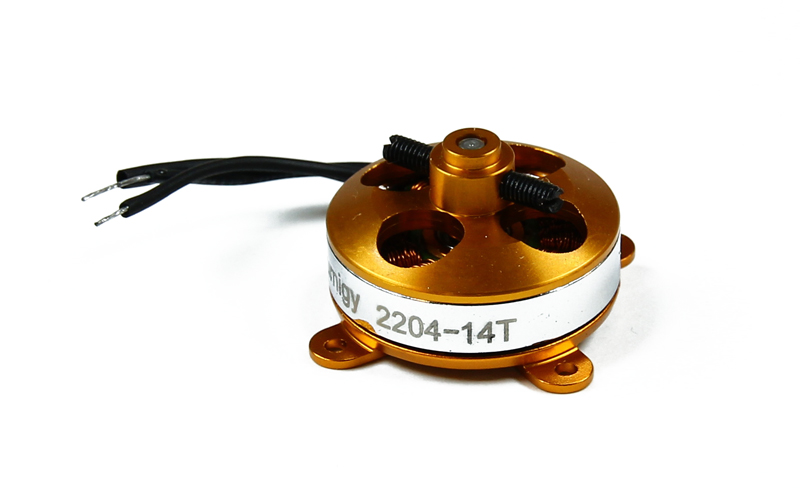
\includegraphics[scale=0.4]{figures/Motors.jpg}
\caption{Motors purchased from \textit{http://www.rcflight.se}}
\label{fig:Motors}
\end{figure}

\section{Design of the System}
%Explain the preliminary design including block diagrams, schematics, drawings, etc.

The functioning of the MCC subsystem is shown in the Figure \ref{fig:design_block}. The transceiver consists of 2.4 Ghz transmitter and receiver. The receiver gets the motor speed control commands to the ESC which in turn actuate the motor to the desired speed.

\begin{figure}[bht]
\centering
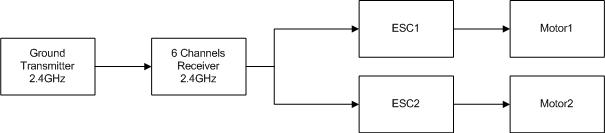
\includegraphics[scale=0.8]{figures/blockdiagram.jpg}
\caption{Block Diagram of the MCC Subsystem}
\label{fig:design_block}
\end{figure}

%\subsection{Software Structure}
%Explain the software structure (if relevant), including block diagrams, flowcharts, hierarchical structure, etc.

%some text...

%\begin{figure}[bht]
%\centering
%
\includegraphics[scale=0.5]{figures/Drawing1}
%\caption{Software structure}
%\label{fig:some_reference}
%\end{figure}


\subsection{Trade-Off Analysis of Concepts}
%Which design concepts are considered? - What are the advantages/disadvantages for each concept?

For the tranceiver system the available options are to use
\begin{itemize}
\item A 72 Mhz transceiver system that uses Amplitude/Frequency Modulation
\item A 2.4 Ghz tranceiver system that uses Spread Spectrum Technology
\end{itemize}

\begin{center}
\begin{table}[bht]
\rowcolors{3}{tableshade}{white}
\begin{tabular}{||l l l||}
\hline\hline
\textbf{Parameter:} &  \textbf{2.4 Ghz Tranceiver} & \textbf{72 Mhz Tranceiver}\\ 
\hline
Frequency Used & 2.4 Ghz & 72 Mhz \\
Crystal Used & No & Yes \\
Change in Frequency & On next power up & By changing the crystal \\
Ability to transmit through obstacles & Weak & Very Good\\
Band Width & Wide & Narrow\\
Date Rate & High & Low\\
Power Usage & Less & More\\
RF Noise Immunity & Very Good & Less \\
\hline
\end{tabular}
\caption{Trade off analysis}
\label{tab:TradeOff}
\end{table}
\end{center}

It is clear from the Table \ref{tab:TradeOff}, that a 2.4 GHz Tranceiver System is a clear winner for chosen application. The only disadvantage of using a 2.4 Ghz tranceiver system is that the receiver should have really good batteries and the voltage should be maintained at a paritcular level. The reason being that there are small processors in the transmitter and receiver that carry out many complex calculation every second without mistake. These processors require constant steady supply of current to work properly. If there is an interruption in the supply current of the receiver then there would be problems with the communication channel.

The speed of the motor can be controlled by the following methods:
\begin{itemize}
\item Use a commercial off the shelf Electronic Speed Controller(ESC) for each motor.
\item Build a Motor Speed Controller using a microprocessor.
\end{itemize}

The primamry advantage of using commercial off the shelf Electronic Speed Controller is the ease of use. This would reduce the development cycle to a large extent. The disadvantage of using it is no scalability i.e. function like autonomous control and telemetery and telecommanding are not possible.

\subsection{Argumentation for Chosen Concept(s)}
%Why is the chosen concept selected?

The 2.4 Ghz tranceiver system would be used for communication. The transceiver used 2.4 Ghz frequency band and uses the spread spectrum technology for transmission of signals. This helps in removing all interfering frequencies caused by other electronic equipments and this helps in having a better communication channel. The other major advantage of using this tranceiver using spread spectrum technology is that the communication channel would not be affected even by someone using the same frequency band.

Commercial off the shelf Electronic Speed Controllers would be used to control the speed of the motors because of time constraint in the project. If time permits it would be desirable to build a speed controller with the help of microprocessor.

\subsection{Feasibility Study of Concept(s)}
%How feasible is it to successfully implement the chosen concept? – Which potential issues/challenges might occur?

The important part in the communication part of the subsystem is deciding upon tranceiver system which would allow bidirectional control of the motor. Since tranceiver is commercial of the shelf, configuring it would be a short task.
Again in the case of motor speed control, choosing the correct ESC and motor combo is the most important task and given maximum time after which assembly is relatively easier and less time consuming.

\subsection{Telemetry and Telecommands}
%What telemetries/telecommands are required/useful for the subsystem? – What data rates/sizes are required?

If time permits, it would be desirable to have a microprocessor for telecommanding and telemetry  which is listed in Table \ref{tab:Telemetry}

\begin{table}[h]
\centering
\begin{tabular}{|l|l|l|}
\hline
\textbf{Telemetry} & \textbf{Data rate/frequency} & \textbf{Data size} \\
\hline
Battery voltage & Every 30 sec & 1 byte \\
\hline
Solar array temperature & Every 30 sec & 1 byte\\
\hline
Solar array voltage & Every 1 sec(MPPT Performance) & 2 bytes\\
\hline
Solar array temperature & Every 1 sec ( MPPT Performance & 2 bytes\\
\hline

\end{tabular}
\caption{Telemetry}
\label{tab:Telemetry}
\end{table}

